\documentclass[10pt,twocolumn,letterpaper]{article}

\usepackage{cvpr}
\usepackage{times}
\usepackage{epsfig}
\usepackage{graphicx}
\usepackage{amsmath}
\usepackage{amssymb}
\usepackage{subfigure}

% Include other packages here, before hyperref.

% If you comment hyperref and then uncomment it, you should delete
% egpaper.aux before re-running latex.  (Or just hit 'q' on the first latex
% run, let it finish, and you should be clear).
\usepackage[breaklinks=true,bookmarks=false]{hyperref}

\cvprfinalcopy % *** Uncomment this line for the final submission

\def\cvprPaperID{****} % *** Enter the CVPR Paper ID here
\def\httilde{\mbox{\tt\raisebox{-.5ex}{\symbol{126}}}}

% Pages are numbered in submission mode, and unnumbered in camera-ready
%\ifcvprfinal\pagestyle{empty}\fi
\setcounter{page}{1}
\begin{document}

%%%%%%%%% TITLE
\title{Praktikum: Virtual Neurorobotics in the Human Brain Project}

\author{Marie Bommersheim, Rafael K\"ubler, and Simon Reinkemeier\\
FZI Forschungszentrum Informatik\\
Karlsruhe\\
%{\tt\small firstauthor@i1.org}
% For a paper whose authors are all at the same institution,
% omit the following lines up until the closing ``}''.
% Additional authors and addresses can be added with ``\and'',
% just like the second author.
% To save space, use either the email address or home page, not both
%\and
%Second Author\\
%Institution2\\
%First line of institution2 address\\
%{\tt\small secondauthor@i2.org}
}

\maketitle
%\thispagestyle{empty}

%%%%%%%%% ABSTRACT
\begin{abstract}
   
\end{abstract}

%%%%%%%%% BODY TEXT
\section{Introduction}

The aim of our Praktikum is to let the robot arm learn how to throw a cylinder as far away from the table as possible. The robot arm and the cylinder are shown in figure \ref{fig:challenge}.

\begin{figure}
	\begin{center}
		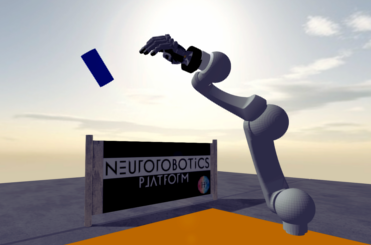
\includegraphics[width=0.4\textwidth]{hbpprak_2018}
	\end{center}
	\caption{The robot arm throwing the cylinder away from the table.}
	\label{fig:challenge}
\end{figure}

Sections \ref{sec:EA} and \ref{sec:MCMC} describe algorithms for solving optimization problems in general. Sections \ref{sec:PrepareHit}, \ref{sec:Throw}, and \ref{sec:Windup} describe our approaches for solving the Praktikum challenge.


\section{Evolutionary Algorithms} \label{sec:EA}

Evolutionary algorithms are population-based metaheuristics \cite{EA}. Metaheuristics are methods for solving optimization problems by iteratively improving candidate solutions in relation to a given quality measure.
Population-based metaheuristics use populations of multiple solutions and iteratively change populations to find a good solution.
An evolutionary algorithm is based on a population $P$ of possible solutions $e_i \in P$ for the optimization problem or heuristic to be solved. A solution is also referred to as an individual in the context of population-based metaheuristics.

In general, evolutionary algorithms consist of the following steps \cite{EA}:

\begin{enumerate}
\item Initialization: The initial population of individuals is generated randomly.

\item Evolutionary process: The individuals are evaluated by calculating their fitness. Therefore a fitness function is needed.
According to their fitness, some of the individuals are selected to be the parents of the following generation.
Then a process with reproduction, recombination, and mutation starts - similar to biological processes.
The parents are being recombinated and the resulting individuals are mutated to form the offspring of the current generation.
These steps are being repeated until a new population of individuals is generated. The parents are also added to the new population. This new population substitutes the old population and the process is repeated until an abort criterion is fulfilled  (see figure \ref{fig:EA}).

\item The best individual is selected.
\end{enumerate}


\begin{figure}
	\begin{center}
		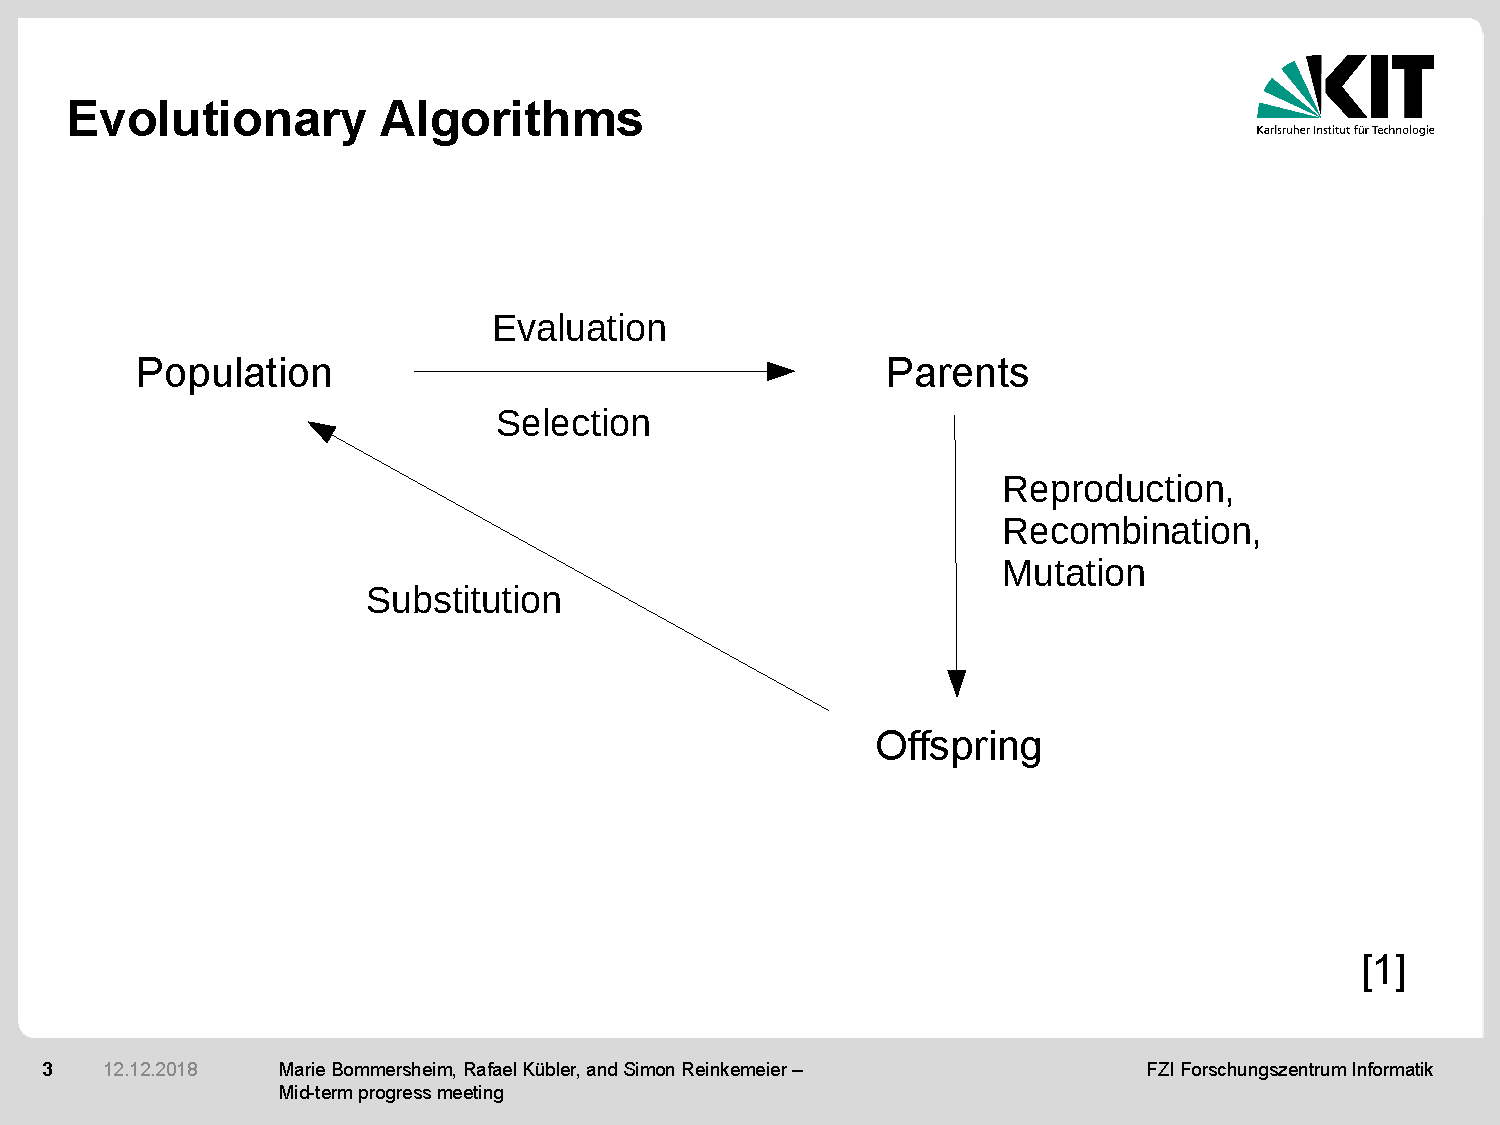
\includegraphics[trim = 2.2cm 6cm 4.1cm 6cm, clip, width=0.4\textwidth]{EA}
	\end{center}
	\caption{Evolutionary algorithms, adapted from \cite{EA}}
	\label{fig:EA}
\end{figure}

\section{Monte Carlo Markov Chain} \label{sec:MCMC}

Monte Carlo Markov Chain algorithms can be used for hard optimization problems. The idea is to construct a Markov Chain that generates samples such that more time is spent (more samples are evaluated) in the most interesting regions of the state space (see figure \ref{fig:MCMC1}) \cite{MCMC}. The decision to accept or reject a proposal to go from Point 1 to Point 2 is based on the ratio of posterior densities of the two points: uphill steps are always accepted, small downhill steps are usually accepted but huge downhill steps are almost never accepted (see figure \ref{fig:MCMC2}). 


\begin{figure}
	\begin{center}
		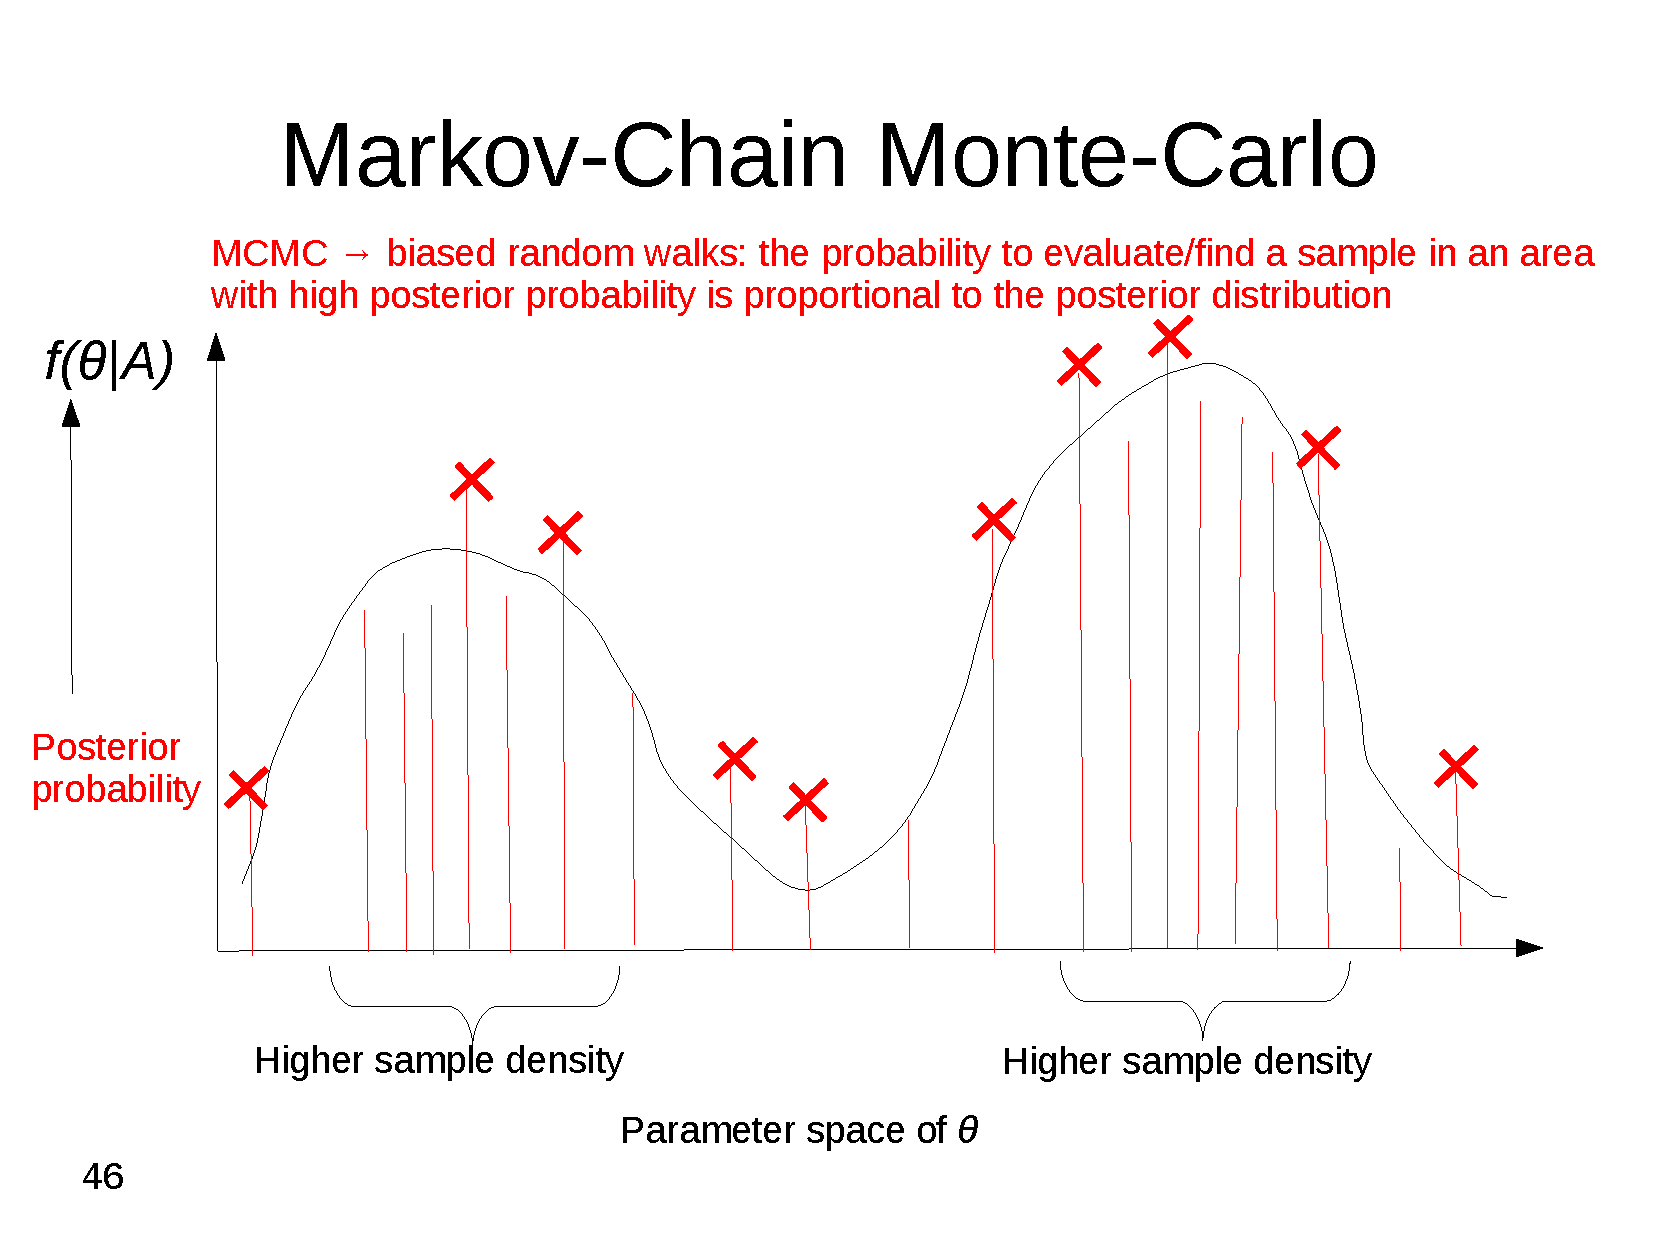
\includegraphics[trim = 0cm 1.5cm 1cm 5.4cm, clip, width=0.4\textwidth]{lecture12-seiten-46}
	\end{center}
	\caption{The probability to evaluate or find a sample in an area with high posterior probability is proportional to the posterior distribution, from \cite{MCMC}}
	\label{fig:MCMC1}
\end{figure}

\begin{figure}
	\begin{center}
		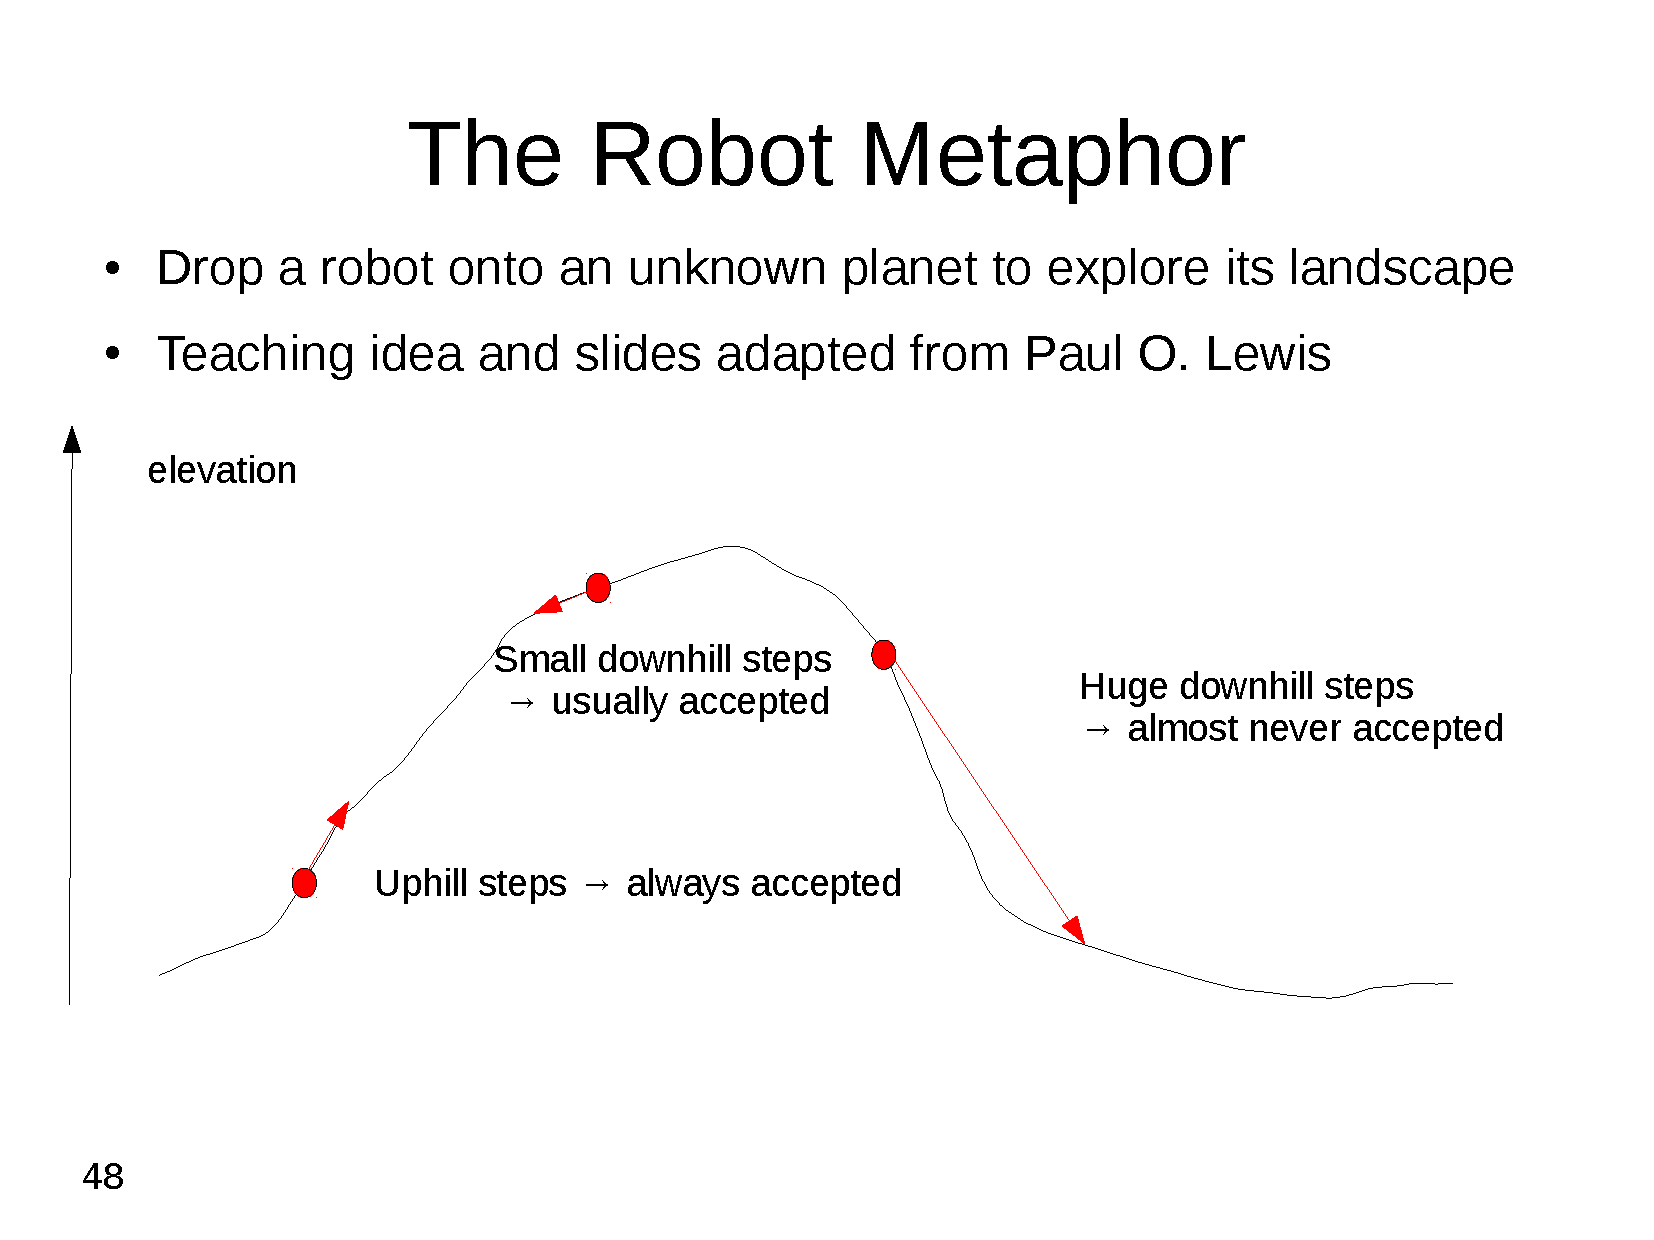
\includegraphics[trim = 0cm 4cm 1cm 7cm, clip, width=0.4\textwidth]{lecture12-seiten-48}
	\end{center}
	\caption{The decision to accept or reject a proposal to go from Point 1 to Point 2 is based on the ratio of posterior densities of the two points/samples, from \cite{MCMC}}
	\label{fig:MCMC2}
\end{figure}


\section{Prepare and Hit} \label{sec:PrepareHit}

The first approach is to let the robot arm hit the cylinder away from the table. Therefore, the movement is divided into three phases: reset, prepare, and hit. The phases are implemented as states using the state machine editor.

\subsection{Hard-coded movements}

At first, the movements are hard-coded:

\begin{itemize}
\item Reset: Moves the arm in an upright position and puts the cylinder on the top right corner of the table (as seen from the robot arm).
\item Prepare: Moves the arm in an horizontal position next to the cylinder (on the left side of the cylinder as seen from the robot arm).
\item Hit: The arm moves towards the cylinder and knocks it off the table.
\end{itemize}

\subsection{Hit movement improved} 

This approach also has the aim of knocking the cylinder off the table, however, the hit movement is not hard-coded but learned using an evolutionary algorithm. The reset and prepare phases are taken from the hard-coded approach.
The evolutionary algorithm which is used to let the robot learn the hit movement is described below: 

An individual of each generation consists of an array of six components (genes) that represent the joints of the robot. The start array is defined as $\begin{bmatrix}
				1 & 1 & 1 & 1 & 1 & 1
				\end{bmatrix}$.
To generate the initial population of ten individuals the start array is mutated by adding random values between $\{-0.1,0.1\}$ to each component.
Computing the next generation consists of three steps:
\begin{enumerate}
\item Selection: The mating pool of four parents is created by selecting the individuals with the highest fitness. The fitness is calculated using the difference between the initial and the end position of the cylinder after knocking it off the table.

\item Mating: In this algorithm, the parents are carried over to the next generation. The recombination process uses one-point crossovers. 

\item Mutation: The offspring is mutated by adding a randomly calculated value between $\{-0.5,0.5\}$ to each component.
\end{enumerate}

These steps are repeated and after ? generations the winner is selected.

\subsection{Prepare and Hit movement improved} 

This approach also uses an evolutionary approach to knock the cylinder off the table. In this approach both the prepare and the hit movement are learned. The reset movement is taken from the hard-coded approach. The evolutionary algorithm is the same as in the previous subsection but with a different start array. 

The start array is a combination of the prepare and the hit movement. It is  created by appending the hit array, given as  
$\begin{bmatrix}
-0.45 &  -0.9 & 0.9 & 0 & 0 & -0.5
\end{bmatrix}$ 
to the prepare array, also given as
$\begin{bmatrix}
-0.45 &  -0.9 & 0.9 & 0 & 0 & -0.5
\end{bmatrix}$.
In this approach, the start pool consists of 15 individuals which are generated from the start array by adding random values between $\{-0.25,0.25\}$ to each component. The mating pool consists of three parents.
The evolutionary algorithm is executed as in the previous approach (with the described changes).

It is repeated for eight generations. 


\section{Prepare, Grasp, and Throw} \label{sec:Throw}

The second approach uses grasp and throw phases to throw the cylinder away from the table. The reset and prepare phases are taken from the first approach and the hit phase is replaced by grasp and throw phases.

\subsection{Hard-coded movements}

At first, the movements are hard-coded.

\begin{itemize}
\item Reset: Moves the arm in an upright position and puts the cylinder on the top right corner of the table (as seen from the robot arm).
\item Prepare: Moves the arm next to the cylinder (on the left as seen from the robot arm).
\item Grasp: Moves the fingers of the robot hand around the cylinder in order to grab it.
\item Throw: With high acceleration, the arm moves backwards beyond the vertical position and the hand opens to throw the cylinder away.
\end{itemize}


\subsection{Throw movement improved} 

This section describes two different ideas to optimize the throw movement. In both approaches the aim is to let the robot learn which movement is best to throw the cylinder as far away from the table as possible.

\subsection{Evolutionary Approach} \label{subsec:EA}

This approach uses the phases from the second approach. The reset, prepare, and grasp are still hard-coded as in the second approach. The throw phase is trained using an evolutionary algorithm. 


\subsection{Markov Chain Monte Carlo Approach} \label{subsec:MCMC}

This approach also uses the phases from the fourth approach. The reset, prepare, and grasp are still hard-coded as in the second approach. The throw phase is trained using a Markov Chain Monte Carlo algorithm. 


\section{Prepare, Grasp, Windup, and Throw} \label{sec:Windup}

{\small
\bibliographystyle{ieee}
\bibliography{egbib}
}

\end{document}
